\chapter{Tactics\label{chap:strategy}}
For Nx1, press the charged attack button when it's full, and try not to get hit.
This chapter's remainder addresses 3x3.
Three subsequent chapters cover team selection, but the topics are intertwined.
A Trainer's Pokémon enable tactics, and tactics guide Pokémon selection.

One of the greatest advantages one can gain is knowledge.
Know Pokémon well, especially those on your team and those you regularly see.
Know what moves they can learn, and how hard they throw them (Power and $\mathit{Eff_A}$).
Knowing their bulk ($\mathit{Eff_D}$ times MHP) can help decide which charged attack to use.
Know type relations cold, and be able to calculate type effectiveness on the fly.
The flipside of this is exploitation of ignorance.
Opposing Trainers are less likely to know Pokémon outside the ``meta'',
 especially those with uncommon typings.
A Pokémon can only know two charged attacks at a time, but if
 chosen from a move pool of three or more charged, even an informed opponent
 can't know what's coming until it's thrown.

\begin{tipbox}[title=A tip regarding battle UI]
Without sufficient energy, pressing the charged attack control employs a fast attack.
If you know you want to throw a charged attack as soon as possible, press its control until thrown.
\end{tipbox}

Take two charged attacks having equal power-per-energy and type, but different power.
The attack delivering more power (and requiring more energy) is beneficial
 when it can achieve a knockout in one hit, but the attack with less power cannot.
This can happen when a new opponent is subbed in, or when the Pokémon is brought back
 after having been subbed out with significant charge.
It also benefits from only one application of the floor function.
Otherwise, the cheaper attack deals comparable damage over time, but deals a portion
 of it earlier, while being less vulnerable to shielding.

Having two charged attacks is a tremendous advantage over only one.
If they are different types, you can gain type advantage over a wide range of opponents.
Since you choose which one to throw on the fly, resistances are much less of a concern.
Their only disadvantage is expense.
A second attack costing 50,000 Stardust is the equivalent of powering up from level 27.5 to 31,
 eleven half-levels.
A 100,000 Stardust second attack is about one-fifth the cost of going from level 1 to 50.

Change to Damage inflicted by an effective Attack is at least 60\%.
Change to Damage inflicted by an ineffective Attack may be as
 low as 37.5\%.
It is probably worth accepting an ineffective Fast Attack if it
 enables an effective Charged Attack, so long as you actually
 get that Charged Attack off.

\subsection{Catching charged attacks}
When a Pokémon drops to very low health (one or two more fast attacks will knock
 them out), they can be subbed out.
Later, when you know a charged attack to be imminent, bring them back in.
If the charged attack is spent knocking out the original Pokémon, its total
 damage is greatly lessened, and you can immediately return to the Pokémon
 you had up.
If you can get an effective fast attack out of the sacrifice, all the better.
This requires sufficient time between the sub out and the catch, and that the
 opponent doesn't knock out your sacrifice Pokémon with fast attacks.

\subsection{Saving charged attacks}
If your Pokémon has almost enough energy to throw a charged attack, but is close to fainting, it can be useful to sub them out.
When they come back, the situation might have changed so that they can get the attack off,
 rather than wasting the builtup energy.
A downside is that an incoming charged attack will probably inflict more total
 damage on a healthy Pokémon than one with little HP to lose.

\subsection{Charged move subterfuge}
It's best to keep an opponent guessing as to your charged moves.
With two moves, an opponent rarely knows which is coming with certainty.
Even with a single move, there is some room for deception.
By holding onto a charged attack longer than necessary, a Pokémon can build
  up energy towards a subsequent attack, and hint towards an attack
  that requires more energy (and thus presumably packs more power).
An opponent that would have absorbed the relatively weak charged attack
  might be induced to blow a shield instead.
This can be particularly effective when the opponent can be drawn down to low HP
  and has one shield left.
The charged attack comes, and is mistaken for a very powerful attack.
A shield is deployed, with the reasoning that the attacked Pokémon can
  do substantial damage with their remaining health, as there isn't
  enough time for a second attack to be charged.
Instead, a second attack comes almost immediately; the Pokémon goes
  down by necessity, and no shields remain.

\subsection{Substitutions\label{subsec:substitutions}}
When the active Pokémon is knocked out, the Trainer selects an unfainted
  Pokémon to replace it (if there is only one such Pokémon, it comes in
  automatically; if there are none, the match is over).
Before a knockout, the Trainer can call for a substitution using any
  unfainted Pokémon.
This starts a substitution cooldown timer of fifty seconds; the Trainer
  cannot perform an early substitution during this time.
Under what circumstances ought early substitutions be made?
Remember that subbing out a Pokémon removes all buffing (\autoref{sec:buffs})
  active for that Pokémon (though not buffs it effected on the opponent).

``Super Effective!'' over one's Pokémon is a frightening message.
It is natural to want to pull them out, ideally bringing in a teammate resistant
  to the revealed opponent's attacks and effective against their typing.
If the opponent can freely substitute, and has a counter to the Pokémon brought in,
  our Trainer is in a world of shit.
Their substituted Pokémon is going to get cooked, and it is unlikely to inflict much damage on the countering Pokémon.
Furthermore, the original threat is still lurking, our original Pokémon is still at a disadvantage,
 and we cannot sub further.
There's no faster way to lose a match.
How, then, to deal with a highly disadvantageous initial matchup?

One can always accept the loss of their lead Pokémon, trying to take some shields and HP with them.
This is not unreasonable if the Trainer has a strong counter at position two or three
  that can come out and mow down the initial Pokémon.
The opponent will of course be able to bring in their own counter when their lead goes down.
The opponent might substitute immediately, protecting their lead (and any charged energy); the Trainer will be able to substitute in turn, possibly locking in a mismatch.
Two Trainers enter a match knowing nothing of the other team's composition.
Losing a Pokémon has the silver lining of freely choosing among your remaining team,
  while knowing at least one member of the opposition.
Substitution has the same benefit.
A chained team, where each Pokémon hard counters the counter of another, can accept such sacrifices.

If the Pokémon brought in is particularly resilient to damage, it might be unlikely that
 the opponent has a good counter available.
By that logic, why not use such a Pokémon as lead, and make the substitution unnecessary?
The lead goes in completely uncertain of their opponent (though the Trainer might have suspicions).
Their charged attacks can always be shielded.
For this reason, I prefer a lead with minimal weaknesses (even if it means few resistances),
 strong fast attacks (perhaps at the expense of energy) with few resistances (even if it means
 few strengths), and low cost charged attacks (despite low power). 
Dragon and Ghost are obviously good candidates here.
Water has some of the best attacks, and several attractive strengths, but Electric and
 especially Grass counters can wipe out Water.
Grass pairs well with Water, the two eliminating most of the other's weaknesses;
 don't sleep on Ludicolo.
Take a look at \autoref{table:defenders}, and familiarize yourself with the first
 and second pages.
I like a lot of hit points in my lead, as they won't be dealing extreme damage.

The intended third Pokémon is coming into a situation with minimal shields available
 to either Trainer.
There's nothing they can do about a mismatch.
They're almost certain to get hit hard, and likely to get their charged attacks in.
Here I don't care about weaknesses; the opponent has limited substitution potential,
 and I don't expect to be around very long anyway.
I want lots of attack---Shadow Pokémon are useful here---and fast attacks that quickly enable my powerful charged attacks.
This Pokémon absolutely must have two strong attacks of different type; it's essential that the charged attack not be resisted.
It's best if they both have STAB\@.
The overpower of charged attacks relative to stamina makes trying to win this via defense a bad idea.

Substituting out a Pokémon with sufficient energy for a charged move (or even two) is a powerful technique.
By doing so, a Trainer has more control over when to use the accumulated energy.
Why waste a knockout blow on an opponent that's already on the ropes?
This can be particularly useful when a fast move is very effective against the current opponent,
 but your charged move is not.
Save that energy for a more profitable matchup.
Of course, the Pokémon you would have knocked out might get a charged attack off on your sub,
 and/or a hard counter might be brought in:
 this is a gamble until you know the opponent's full lineup.
On this note, when deciding whether to shield, be sure to account for built up energy on the opponent's bench.

\subsection{Charged move timing\label{subsec:cmt}}
Recall from \autoref{chap:battle} that charged attacks:
\begin{itemize}
\item inflict damage on the turn thrown,
\item conclude an opponent's fast attack, and
\item inflict damage prior to said fast attack.
\end{itemize}
A result of these mechanics is that on the turn following a charged attack,
 both Pokémon are ready to throw a new attack.

Pokémon A concludes their $T_A$-turn fast attack, and has sufficient energy to throw a charged attack.
If Pokémon B has a one-turn fast attack, everything is very simple;
 A can throw charged attacks whenever they'd like.
If Pokémon B is in the middle of a $T_B$-turn fast attack, with $R$ turns remaining,
 and $T_A < R$, throwing the charged attack constitutes a blunder\footnote{Unless it wins the match.}.
It brings Pokémon B's fast attack to an early conclusion, leaving them ready to start a new attack.
If instead Pokémon A runs a fast attack, that attack completes before Pokémon B's, inflicting damage and generating energy.
The charged attack can then be thrown.
In the extreme case of facing an attack of five turns while using one of a single turn,
  you can get four attacks in before optimally launching the charged attack.

Let's assume Pokémon A employs Poison Jab, a two-turn fast attack.
Pokémon B throws five-turn Incinerate at $T_n$.
If Pokémon A throws its charged attack, at $T_{n+1}$ it will have inflicted
  one charged attack, and suffered one fast attack.
Instead, Pokémon A throws Poison Jab, which concludes on $T_{n+1}$, dealing damage and charging energy.
On $T_{n+2}$, Pokémon A launches Poison Jab a second time, concluding on $T_{n+3}$.
Finally, at $T_{n+4}$, Pokémon A throws its charged attack.
The result when $T_{n+5}$ rolls around is that both stand ready to throw new attacks,
  but Pokémon A has the benefit of two extra fast attacks.
Compared to throwing the charged attack prior to $T_{n+4}$,
  Pokémon A has inflicted more damage and built up more energy.
A result: if your fast attack is fewer turns than your opponent's,
 and you're both set to choose attacks,
 \textit{don't throw a charged attack if you expect them to throw a fast attack}.
Go with $\lfloor\frac{T_B}{T_A}\rfloor$ fast attacks first.
Even if you're wrong, and they throw a charged attack, you'll get credit for the fast attack---unless you get knocked out.

Optimal timing requires throwing charged moves only when $R=1$, and continuously throwing fast moves otherwise
 (again, this assumes $T_B > 1$).
This is impossible to do when $T_A$ is a multiple of $T_B$\footnote{In my opinion, long fast moves are an advantage against weak competition, and a disadvantage
 against strong competition. Weak competition is more likely to throw early, giving up fast attacks. Strong competition
 won't do so, and you never get those attacks.}.
The interesting case is when $1 < R \le T_A$ (if $1=R$, the charged attack is optimally timed; if $R > T_A$, throw a fast attack).
Replace Poison Jab with Astonish (three turns).
It throws Astonish at $T_n$, concluding at $T_{n+2}$.
Throwing Astonish a second time won't see it conclude until $T_{n+5}$.
Assume Pokémon B throws a second Incinerate at $T_{n+5}$.
The time between charged attacks can be thought of as a ``period''
 in which each Pokémon lands some number of fast attacks.
A Trainer wants to maximize the ratio of their fast attacks to their opponent's.
If Pokémon A throws its charged attack at $T_{n+6}$, at $T_{n+7}$ Pokémon B has landed two Incinerates
  against two Astonishes and a charged attack.
A charged attack at $T_{n+3}$ would lead to one Incinerate against one Astonish
  and a charged attack.
Pokémon A catches up at $T_{n+9}$, when it has thrown three attacks, and Pokémon B is
  completing its second.
This 3:2 ratio seems as good as it gets for Pokémon A.
At $T_{n+12}$, we're down to 4:3, and $T_{n+15}$ is 5:4.

\begin{tipbox}[title=Warning! Achtung! \begin{chinese}危险!\end{chinese} ¡Peligro! \begin{japanese}危険!\end{japanese} \textit{Tulaga faigata!}]
I now contradict longstanding claims of the Pokémon GO community, repeated by
  people far more experienced than me.
Nonetheless, I'm pretty sure they're all wrong, and I'm right.
\end{tipbox}
\noindent{}Again and again, one reads that charged moves ought be thrown on the natural last turn of an
 opponent's fast move, lest the opponent gain tempo\footnote{EmpoleonDynamite's ``\href{https://pvpoke.com/articles/strategy/guide-to-fast-move-registration/}{Guide to Fast Move Mechanics}''
 on \href{https://pvpoke.com}{pvpoke.com} (2022), FlarkeFiasco's r/TheSilphArena post ``\href{reddit.com/r/TheSilphArena/comments/fvu62a/charge\_move\_timing\_yes\_it\_really\_does\_matter/}{Charge Move Timing---Yes, it *really* does matter}'' (2020),
 avrip's ``\href{https://pokemongohub.net/post/pvp/mastering-the-turn-system-in-pokemon-go-pvp/}{Mastering the Turn System in Pokémon GO PVP}'' on GOHub (2024),
 and Wallower's YouTube video ``\href{https://www.youtube.com/watch?v=pAtCo8xg700}{GBL Advanced Mechanics 1: Charged Move Timing}'' (2021).}.
But this rule is incomplete.

Pokémon B's fast moves complete on turns $T_{n+5a-1}$ for positive integers $a$.
Pokémon A can throw charged moves on turns $T_{n+3b}$ for non-negative integers $b$.
The rule considers $T_{n+9+15c}$ for non-negative integers $c$ optimal times to throw
 ($T_{n+9}, T_{n+24}, \dots$), and these are indeed \textit{locally} optimal.
At $T_{n+18}$, the ratio is 6:4, the same as 3:2, despite \textit{not} being the last turn of Pokémon B's attack.
And at $T_{n+24}$, the ratio is 8:5, \textit{better} than $T_{n+9}$!
The maxima converge to 5:3.

\begin{figure}
\begin{minipage}{0.5\textwidth}\centering
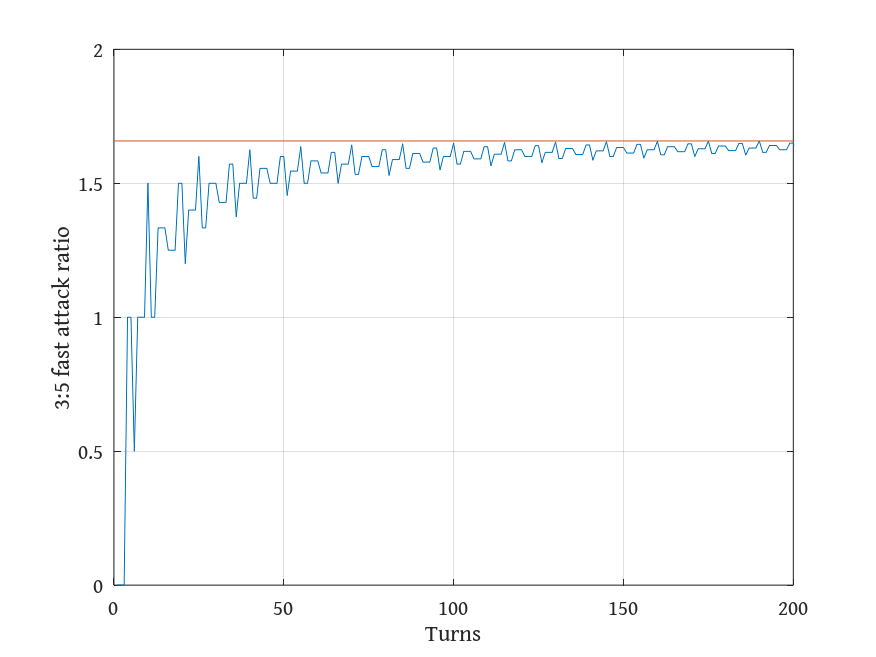
\includegraphics[width=\textwidth,keepaspectratio]{octave/3vs5fastcharged.png}
\end{minipage}
\begin{minipage}{0.5\textwidth}\centering
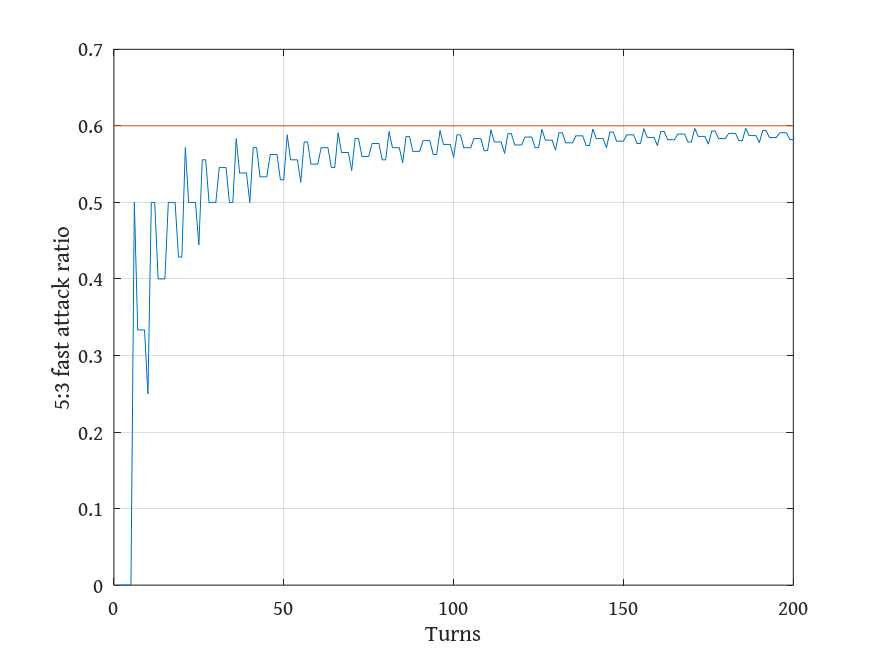
\includegraphics[width=\textwidth,keepaspectratio]{octave/5vs3fastcharged.png}
\end{minipage}
\caption{Ratios of 3- and 5-turn fast moves (200 turns)\label{figure:35ratios}}
\end{figure}

What about Pokémon B\@?
Ideally they get their charged move out at $T_{n+5}$, for a 1:1 ratio.
At $T_{n+10}$ the ratio is 2:4, but at $T_{n+15}$ it is 3:6, despite landing on the first turn of the sixth fast attack.
At $T_{n+20}$ the ratio is 4:7, but it falls back to 5:9 at $T_{n+25}$.
These maxima of course converge to 3:5.

Simply postponing a charged move can be just as or more effective than timing with
  respect to the opponent's fast attack.
Why is this important?
It can be useful to delay a charged attack for any number of reasons.
If Pokémon A was willing to accept a 1.5 ratio, throwing after three Astonish
  attacks suffices, but six works as well, despite not being the last turn of an Incinerate.
No efficiency is lost relative to the three case, though neither three nor six are as
  efficient as 24.
The true maximum efficiency cannot be reached.

\begin{tabular}{lrrrr}
  Turn A throws & $R$ & A fast attacks & B fast attacks & Ratio \\
\Midrule
  0 & 5 & 0 & 1 & 0 \\
  3 & 2 & 1 & 1 & 1\\
  6 & 4 & 2 & 2 & 1\\
  9 & 1 & 3 & 2 & 1.5 \\
  12 & 3 & 4 & 3 & 1.\textoverline{3} \\
  15 & 5 & 5 & 4 & 1.2 \\
  18 & 2 & 6 & 4 & 1.5 \\
  21 & 4 & 7 & 5 & 1.4 \\
  24 & 1 & 8 & 5 & 1.6 \\
  27 & 3 & 9 & 6 & 1.5 \\
  30 & 5 & 10 & 7 & \sim{}1.429 \\
  33 & 2 & 11 & 7 & \sim{}1.571 \\
  36 & 4 & 12 & 8 & 1.5 \\
  39 & 1 & 13 & 8 & 1.625 \\
  $\infty$ & 0 & 5n & 3n & 1.\textoverline{6} \\
\end{tabular}

\begin{tabular}{lrrrr}
  Turn B throws & $R$ & A fast attacks & B fast attacks & Ratio\\
\Midrule
  0 & 3 & 1 & 0 & 0 \\
  5 & 1 & 1 & 2 & 0.5\\
  10 & 2 & 2 & 4 & 0.5\\
  15 & 3 & 3 & 6 & 0.5\\
  20 & 1 & 4 & 7 & \sim{}0.571\\
  25 & 2 & 5 & 9 & 0.\textoverline{5}\\
  30 & 3 & 6 & 11 & 0.\textoverline{54}\\
  35 & 1 & 7 & 12 & 0.58\textoverline{3}\\
  $\infty$ & 0 & 3n & 5n & 0.6 \\
\end{tabular}

If your opponent still has both shields very late in the match, avoid charged attacks entirely.
Two are going to do the minimum single point of damage, and possibly give the opponent a gift of tempo.
